%----------------------------------------------------------------------------------------
%	CHAPTER 4
%----------------------------------------------------------------------------------------

\chapterimage{head1.png} % Chapter heading image

\chapter{Experimenting}

I discovered surfing on the internet a cloud computing software that is free, has data mining algorithms embedded, is specifically developed for Astronomy and is programmed by Caltech, University Federico II and the Astronomical Observatory of Capodimonte. The homepage website, \url{http://dame.dsf.unina.it/index.html}. Well, the platform for testing is ready!, now what? I requested and account and the next day they sent me an acceptance with my user name and my password approved.
I introduced myself to the documentation, the available clustering functions, the manuals for every method, the blogs and discovered that the was one method available that could work with data cubes and do its clustering on every pattern (number in the multidimensional matrix) which was exactly what I needed. The name of this method is ESOM (Evolving Self Organizing Maps) and I read its manual, did some foolish test with all my image and ... never got a result ... the experiment ran forever (more than two weeks), when I realised that this wasn't the best way to tackle this problem I started considering only clustering on the independent images and not in the data cube due to the fact that the dimensionality was immense. So, in the end my selected methods have some results but not all, here is where all the work has to be done, analysed and tested again.

\section{Methods Selected}

\subsection{ESOM, Evolving Self Organizing Maps}
The \emph{official} manual for this method can de found here, \url{http://dame.dsf.unina.it/documents/ESOM_UserManual_DAME-MAN-NA-0021-Rel1.2.pdf}, there you will find a full explanation of the method, the meaning of every variable and the supported file types.

Here is my own explanation of how this particular method works, first of all, can be used as an unsupervised machine learning technique or you can help the algorithm to identify regions an make it a supervised machine learning technique, this type of clustering finds groups of patterns with similarities and preserves its topology, starts with a null network without any nodes and those are created incrementally when a new input pattern is presented, the prototype nodes in the network compete with each other and the connections of the winner node are updated. 

The method is divided in three stages, \emph{Train}, \emph{Test} and \emph{Run}.
The first step to experiment with this method is Train. Here, the important variables to understand an look at are, the learning rate, epsilon and the pruning frequency. It is highly recommendable that you check the DAMEWARE manual for this function, there they will explain in detail the meaning of each on the mentioned variables.

\subsubsection{Expected Results}
	This particular method as I mentioned before supports data cubes and considers as an independent pattern all the  numbers in the multi-dimensional array this means that our clusters are groups of patterns with similar characteristics, that correspond to volumes of similar fluxes of electrons inside the data cube.
    
    The output files from the experiment that will show us our results are, 
    \begin{itemize}
    	\item \emph{E\_SOM\_Train\/Test\/Run\_Results.txt}: File that, for each pattern, 
reports ID, features, BMU, cluster and activation of winner node
		\item \emph{E\_SOM\_Train\/Test\/Run\_Histogram.png}: Histogram of clusters found 
        \item \emph{E\_SOM\_Train\/Test\/Run\_U\_matrix.png}: U-Matrix image 
        \item \emph{E\_SOM\_Train\/Test\/Run\_Clusters.txt}: File that, for each clusters, reports label, number of pattern assigned, percentage of association respect total number of pattern and its centroids. 
        \item \emph{E\_SOM\_Train\_Datacube\_image.zip}: Archive that includes the 
clustered images of each slice of a data cube.\footnote{I have my doubts whether this file is produced or not, in none of my test was produced, you might need to contact the developers and ask about this.}
    \end{itemize}
The file that you will be looking forward to see is the last one, the zip where you will be able to see the slices of the volume, and how the final configuration of the clusters was arranged.

\subsubsection{Failed and still running tests: What no to do and what is still running}
The first tests I did included all the complete data cube, including the areas where data was missing, the images were only re-projected and convolved. That was before realising that outliers might affect the ability of the algorithm to identify the clusters and distract them with noise and missing data. So, the first thing you must NOT do, is to get rid of the outliers when you are training your network, if you ever get to have a well trained network then it might be interesting to learn how the network interacts with noise an outliers, but for now we will help her a bit. 

In table \ref{tab:ds9failed} are the input parameters I used to the failed tests applied in the \emph{raw} data cube, and in table \ref{tab:ds9running} are the input parameters used on experiments that are still running since August 7th, 2014. (I wonder if they will ever end)

\begin{table}[h!]
  \centering
    \begin{tabular}{ c c c c c c }
    \hline\hline
    
    Name & Input nodes & Normalized data & Learning rate & Epsilon & Pruning Frequency\\
    \hline
    
    Train2 & 1 & 1 & 0.3 & 0.001 & 5\\
    Train3 & 1 & 1 & 0.7 & 10 & 100\\
    Train4 & 1 & 1 & 0.95 & 1 & 10\\
    Train5 & 1 & 1 & 0.99 & 0.1 & 10\\
    Train6 & 1 & 1 & 0.01 & 0.01 & 1\\
    Train7 & 1 & 1 & 0.5 & 0.7 & 5\\
    Train8 & 1 & 1 & 0.5 & 0.5 & 7\\
    Train11 & 1 & 1 & 0.25 & 0.00001 & 10\\
    
    \hline
  \end{tabular}
  \caption{This table describes all the failed experiments done in the workspace WFC3 with the \emph{raw} data cube as an input, using the ESOM method in the DAME platform selecting the number 3 as the dataset type and without using a previous configuration file.}
  \label{tab:ds9failed}
\end{table}

\begin{table}[h!]
  \centering
    \begin{tabular}{ c c c c c c }
    \hline\hline
    
    Name & Input nodes & Normalized data & Learning rate & Epsilon & Pruning Frequency\\
    \hline
    
    Train9 & 1 & 1 & 0.3 & 0.0001 & 5\\
    Train10 & 1 & 1 & 0.99 & 0.0001 & 10\\
    Train12 & 1 & 1 & 0.5 & 0.0001 & 5\\
    
    \hline
  \end{tabular}
  \caption{This table describes all the experiments done in the workspace WFC3 that are still running since August 7th, 2014 with the \emph{raw} data cube as an input, using the ESOM method in the DAME platform selecting the number 3 as the dataset type and without using a previous configuration file.}
  \label{tab:ds9running}
\end{table}

Some of the failed experiments had histogram like the one you can see on figure \ref{img:faildtrain2} where the clusters were created but reached a point where the neural network could not define how to differentiate a cluster from another cluster and failed.

\begin{figure}[h!]
	\centering
    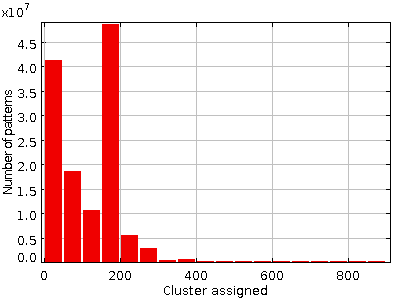
\includegraphics[width=0.47\textwidth]{Histogram_train2.png}
    \caption{In this particular experiment, the neural network failed due to a very low pruning frequency, high number of patterns and all the outliers inclusions.}
    \label{img:faildtrain2}
\end{figure}

Hey, if you were wondering why I always choose to normalize, and one as the input node, well the normalization is due to the fact that I know that the data has, according to its filter, all kinds of ranges of fluxes on every layer which means that the distances between patterns might not be correct, this is a topic you should look into. And for the input node I choose 1 because if I start with any other number the experiment automatically fails, and of course we do not want that.

As I progressed and saw the results and the \emph{log files} in all the failed experiments I decide to try the algorithm on independent layers and see if I could get something. Therefore I selected the H$\alpha$ convolved observation (halpha\_conv.fits) and did some tests on it, table \ref{tab:hafailed} shows the parameters I used for the failed experiments and table \ref{tab:harun} shows the parameters of the still running experiments.

\begin{table}[h!]
  \centering
    \begin{tabular}{ c c c c c c }
    \hline\hline
    
    Name & Input nodes & Normalized data & Learning rate & Epsilon & Pruning Frequency\\
    \hline
    
    TrainHa1 & 1 & 1 & 0.5 & 0.01 & 5\\
    TrainHa2 & 1 & 1 & 0.5 & 0.001 & 5\\
    
    \hline
  \end{tabular}
  \caption{This table describes the failed experiments done in the workspace WFC3 for the \emph{halpha\_conv.fits} file, using the ESOM method for one layer in the DAME platform selecting the number 3 as the dataset type and without using a previous configuration file.}
  \label{tab:hafailed}
\end{table}

\begin{table}[h!]
  \centering
    \begin{tabular}{ c c c c c c }
    \hline\hline
    
    Name & Input nodes & Normalized data & Learning rate & Epsilon & Pruning Frequency\\
    \hline
    
    TrainHa3 & 1 & 1 & 0.5 & 0.0001 & 5\\
    
    \hline
  \end{tabular}
  \caption{This table describes the still running experiments since August 10th, 2014 in the workspace WFC3 for the \emph{halpha\_conv.fits} file, using the ESOM method for one layer in the DAME platform selecting the number 3 as the dataset type and without using a previous configuration file.}
  \label{tab:harun}
\end{table}

My next mental step was to repeat the tests eliminating as many outliers I could reduce, my hypothesis here is that, if I eliminate all the areas where there is missing data and noise, the neural networks will be concentrated only in the patterns I'm interested in clustering and maybe identifying interesting regions that correspond to some known interstellar object. So, what I did was to try the ESOM algorithm with, again, independent images, this time I decided to apply the same experiment to three different layers, H$\alpha$, UV wide and $i$-band. In table \ref{tab:threefail} you can see the parameters of the failed experiments and on figure \ref{img:fail3} there are some of the output histograms. Also, in table \ref{tab:threerun} you can see the input parameters of the still running experiments.

\begin{table}[h!]
  \centering
    \begin{tabular}{ c c c c c c }
    \hline\hline
    
    Name & Input nodes & Normalized data & Learning rate & Epsilon & Pruning Frequency\\
    \hline
    
    Train1 & 1 & 1 & 0.5 & 0.001 & 50\\
    Train2 & 1 & 1 & 0.5 & 0.01 & 50\\
    Train3 & 1 & 1 & 0.5 & 0.1 & 100\\
    Train4 & 1 & 1 & 0.5 & 0.001 & 100\\
    
    \hline
  \end{tabular}
  \caption{This parameters where used in three different workspaces (\emph{halphaCrop, uvwidecrop, ibandcrop}), with their own input file that corresponded to the convolved and cropped observation of each filter (halpha\_conv\_crp.fits, uvwide\_conv\_crp.fits, iband\_conv\_crp.fits), all of the experiments had no previous configuration file and the dataset type was 3 and all failed.}
  \label{tab:threefail}
\end{table}

\begin{figure}[h!]
	\centering
    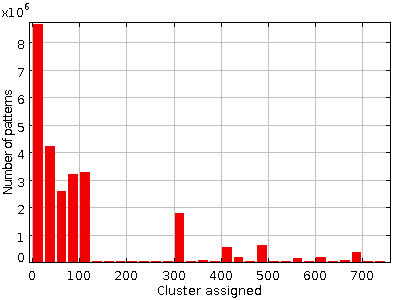
\includegraphics[width=0.31\textwidth]{Histogram-halpha1.png}
    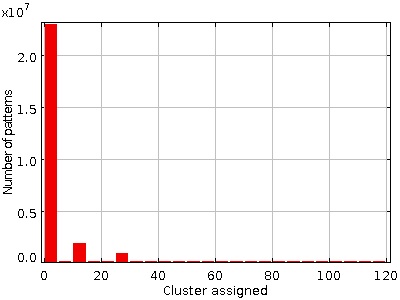
\includegraphics[width=0.31\textwidth]{Histogram-uvwide-2.png}
    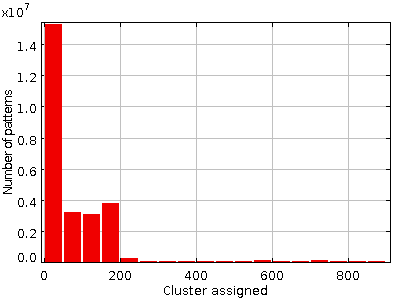
\includegraphics[width=0.31\textwidth]{Histogram-iband3.png}
    \caption{The histogram on the left corresponds to the halpha workspace in Train1, the one on the center to the iband workspace in Train3 and the one on the right to the uvwide workspace in Train2, all of them were failed experiments.}
    \label{img:fail3}
\end{figure}

\begin{table}[h!]
  \centering
    \begin{tabular}{ c c c c c c }
    \hline\hline
    
    Name & Input nodes & Normalized data & Learning rate & Epsilon & Pruning Frequency\\
    \hline
    
    Train5 & 1 & 1 & 0.5 & 0.0001 & 100\\
    Train6 & 1 & 1 & 0.99 & 0.0001 & 75\\

    \hline
  \end{tabular}
  \caption{This parameters where used in three different workspaces (\emph{halphaCrop, uvwidecrop, ibandcrop}), with their own input file that corresponded to the convolved and cropped observation of each filter (halpha\_conv\_crp.fits, uvwide\_conv\_crp.fits, iband\_conv\_crp.fits), all of the experiments had no previous configuration file and the dataset type was 3. The experiments mentioned are still running since August 11th, 2014.}
  \label{tab:threerun}
\end{table}

As you can see, I discovered that if I choose an epsilon of 0.0001 the experiments will be still running, and all of the other variables can be variated like the learning rate and the pruning frequency.

\subsubsection{The big and small re-projected data cube}
After a few days of waiting anxiously for the experiments to end and not getting any new results I decided to test the convolved, cropped and re-projected data cube including all the layers with a fixated pruning frequency of 0.0001, hopping that this time I could get some interesting results. The input parameters for the two experiments I tested can be seen in table \ref{tab:cubeesom}.

\begin{table}[h!]
  \centering
    \begin{tabular}{ c c c c c c }
    \hline\hline
    
    Name & Input nodes & Normalized data & Learning rate & Epsilon & Pruning Frequency\\
    \hline
    
    ESOMtrain1 & 1 & 1 & 0.5/0.75 & 0.0001 & 100\\
    ESOMtrain2 & 9 & 1 & 0.75 & 0.001 & 100\\

    \hline
  \end{tabular}
  \caption{This parameters where used in two different workspaces (\emph{Data Cube, RPDataCube}), the first experiment is still running since August 12th, 2014 and the second failed. The input for the Data Cube workspace corresponds to a 9 layer data cube with no re-projection and the RPDataCube input is the same data cube but re-projected.}
  \label{tab:cubeesom}
\end{table}

As you can see, in the experiment \emph{ESOMtrain2} I tried to start the neural network with 9 nodes (thinking logically as having 9 layers in the data cube) and immediately the experiment failed, so \textbf{do not try to input a number different than one.}

I waited 17 days for the experiments to finish (I did some other stuff in the meanwhile, most of the time learning new things) but I did not get any results so I came up with a different strategy, selecting small data cubes with already identified regions by the NED database. I selected randomly a particular HII region located in RA 204.26971, DEC -29.84933 (See figure \ref{img:h2region}) and centred it in a 605x605 pixels sample.

\begin{figure}[h!]
	\centering
    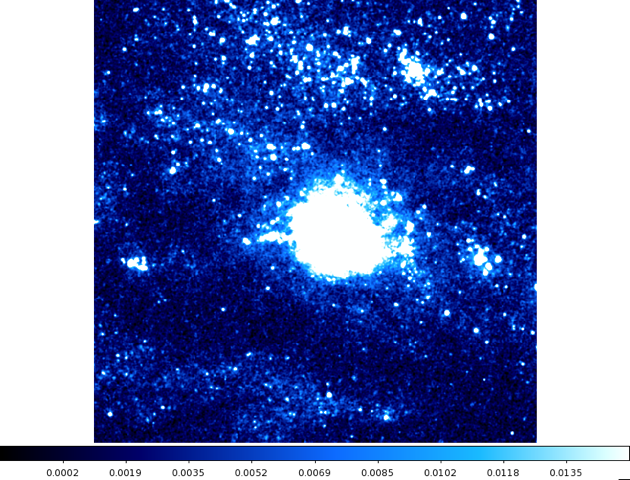
\includegraphics[width=0.52\textwidth]{small_ex.png}
    \caption{Illustration of the randomly chosen HII region for the small sample from the M83 re-projected data cube.}
    \label{img:h2region}
\end{figure}

This time, most of the experiments gave me immediate results failing or finishing. On table \ref{tab:small}, you can see the input parameters and the status of the experiments I tested with the small data cube.

\begin{table}[h!]
  \centering
    \begin{tabular}{ c c c c c c }
    \hline\hline
    
    Name & Normalized & Learning rate & Epsilon & Pruning Frequency & Status\\
    \hline
    
    ESOMtrain1 & 0 & 0.5 & 0.001 & 50 & Running\\
    Train2 & 1 & 0.5 & 0.0001 & 50 & Ended\\
    Train3 & 1 & 0.5 & 0.1 & 50 & Ended\\
    Train4 & 0 & 0.5 & 0.0001 & 50 & Running\\
    Train5 & 0 & 0.95 & 0.0001 & 100 & Running\\
    Train6 & 1 & 0.99 & 0.001 & 50 & Ended\\

    \hline
  \end{tabular}
  \caption{All the mentioned experiment belong to the SmallDataCube workspace, have 3 as data type and one input node, no previous configuration file and the input file is \emph{rp\_small\_datacube.fits}.}
  \label{tab:small}
\end{table}
In this case three of the experiments ended and none of them failed (yet), here I detected that the output file that contains the distributions of the clusters on every layer is missing, but we got some interesting results, in the next figures (\ref{img:smallended},\ref{img:matrixended}) you can appreciate better what I'm taking about.

\begin{figure}[h!]
	\centering
    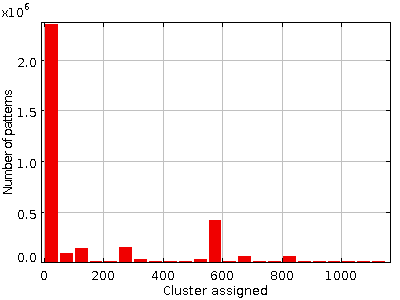
\includegraphics[width=0.31\textwidth]{Small-train2.png}
    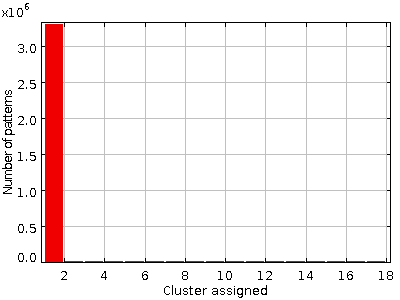
\includegraphics[width=0.31\textwidth]{Small-train3.png}
    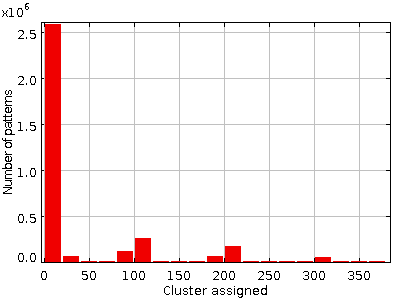
\includegraphics[width=0.31\textwidth]{Small-train6.png}
    \caption{All of the images correspond to histograms of the ended experiments mentioned above in order (Train2, Train3, Train6), as you can see there is a predominance on one of the clusters that can mean that is detecting the HII region or the experiment never started, to understand further the results a visualization of the clusters is needed.}
    \label{img:smallended}
\end{figure}

\begin{figure}[h!]
	\centering
    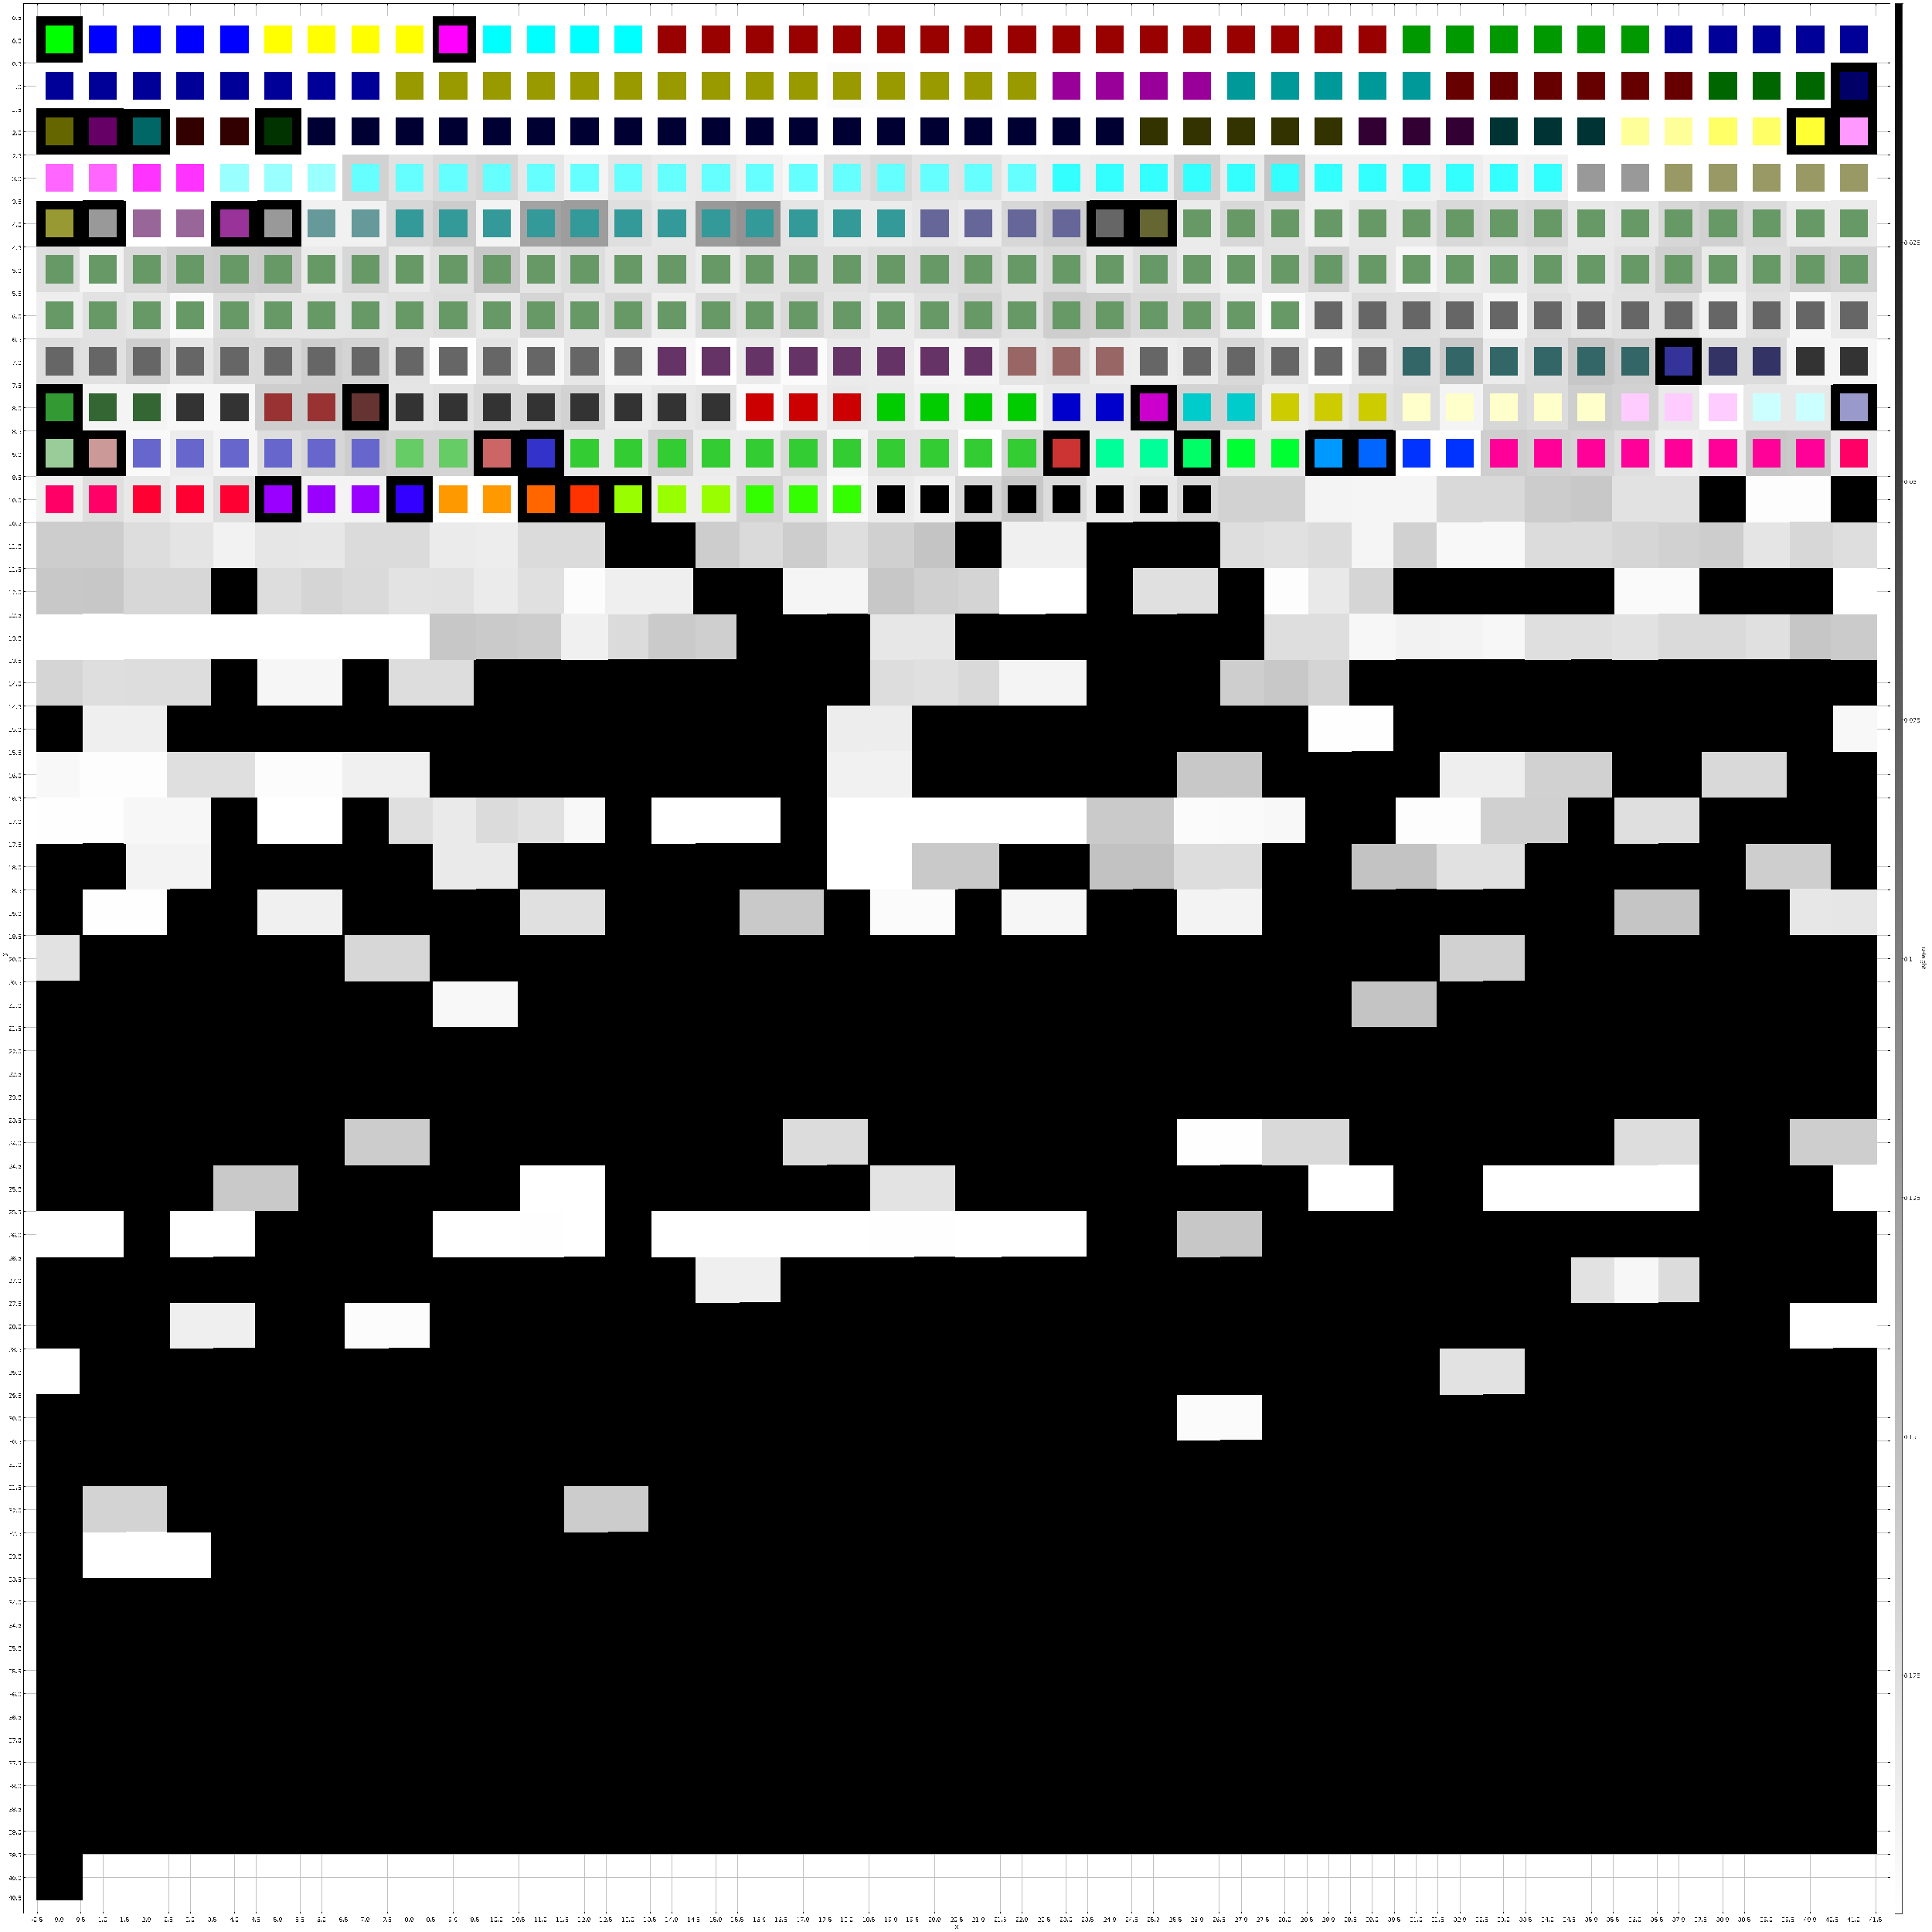
\includegraphics[width=0.31\textwidth]{matrix2-01.png}
    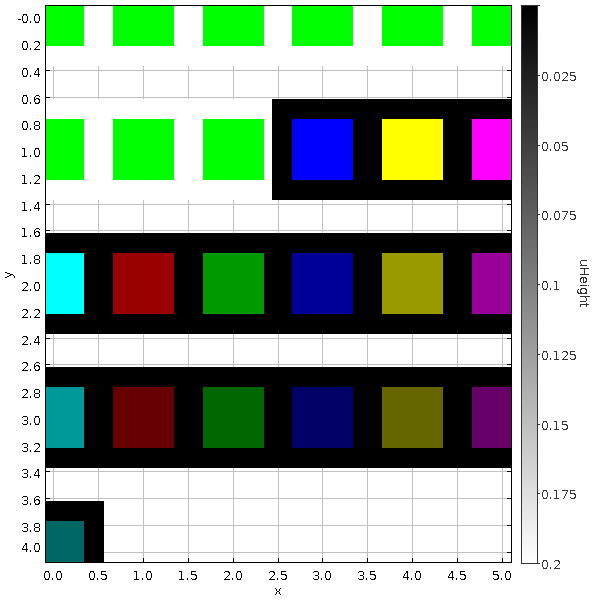
\includegraphics[width=0.31\textwidth]{Small-train3-matrix.png}
    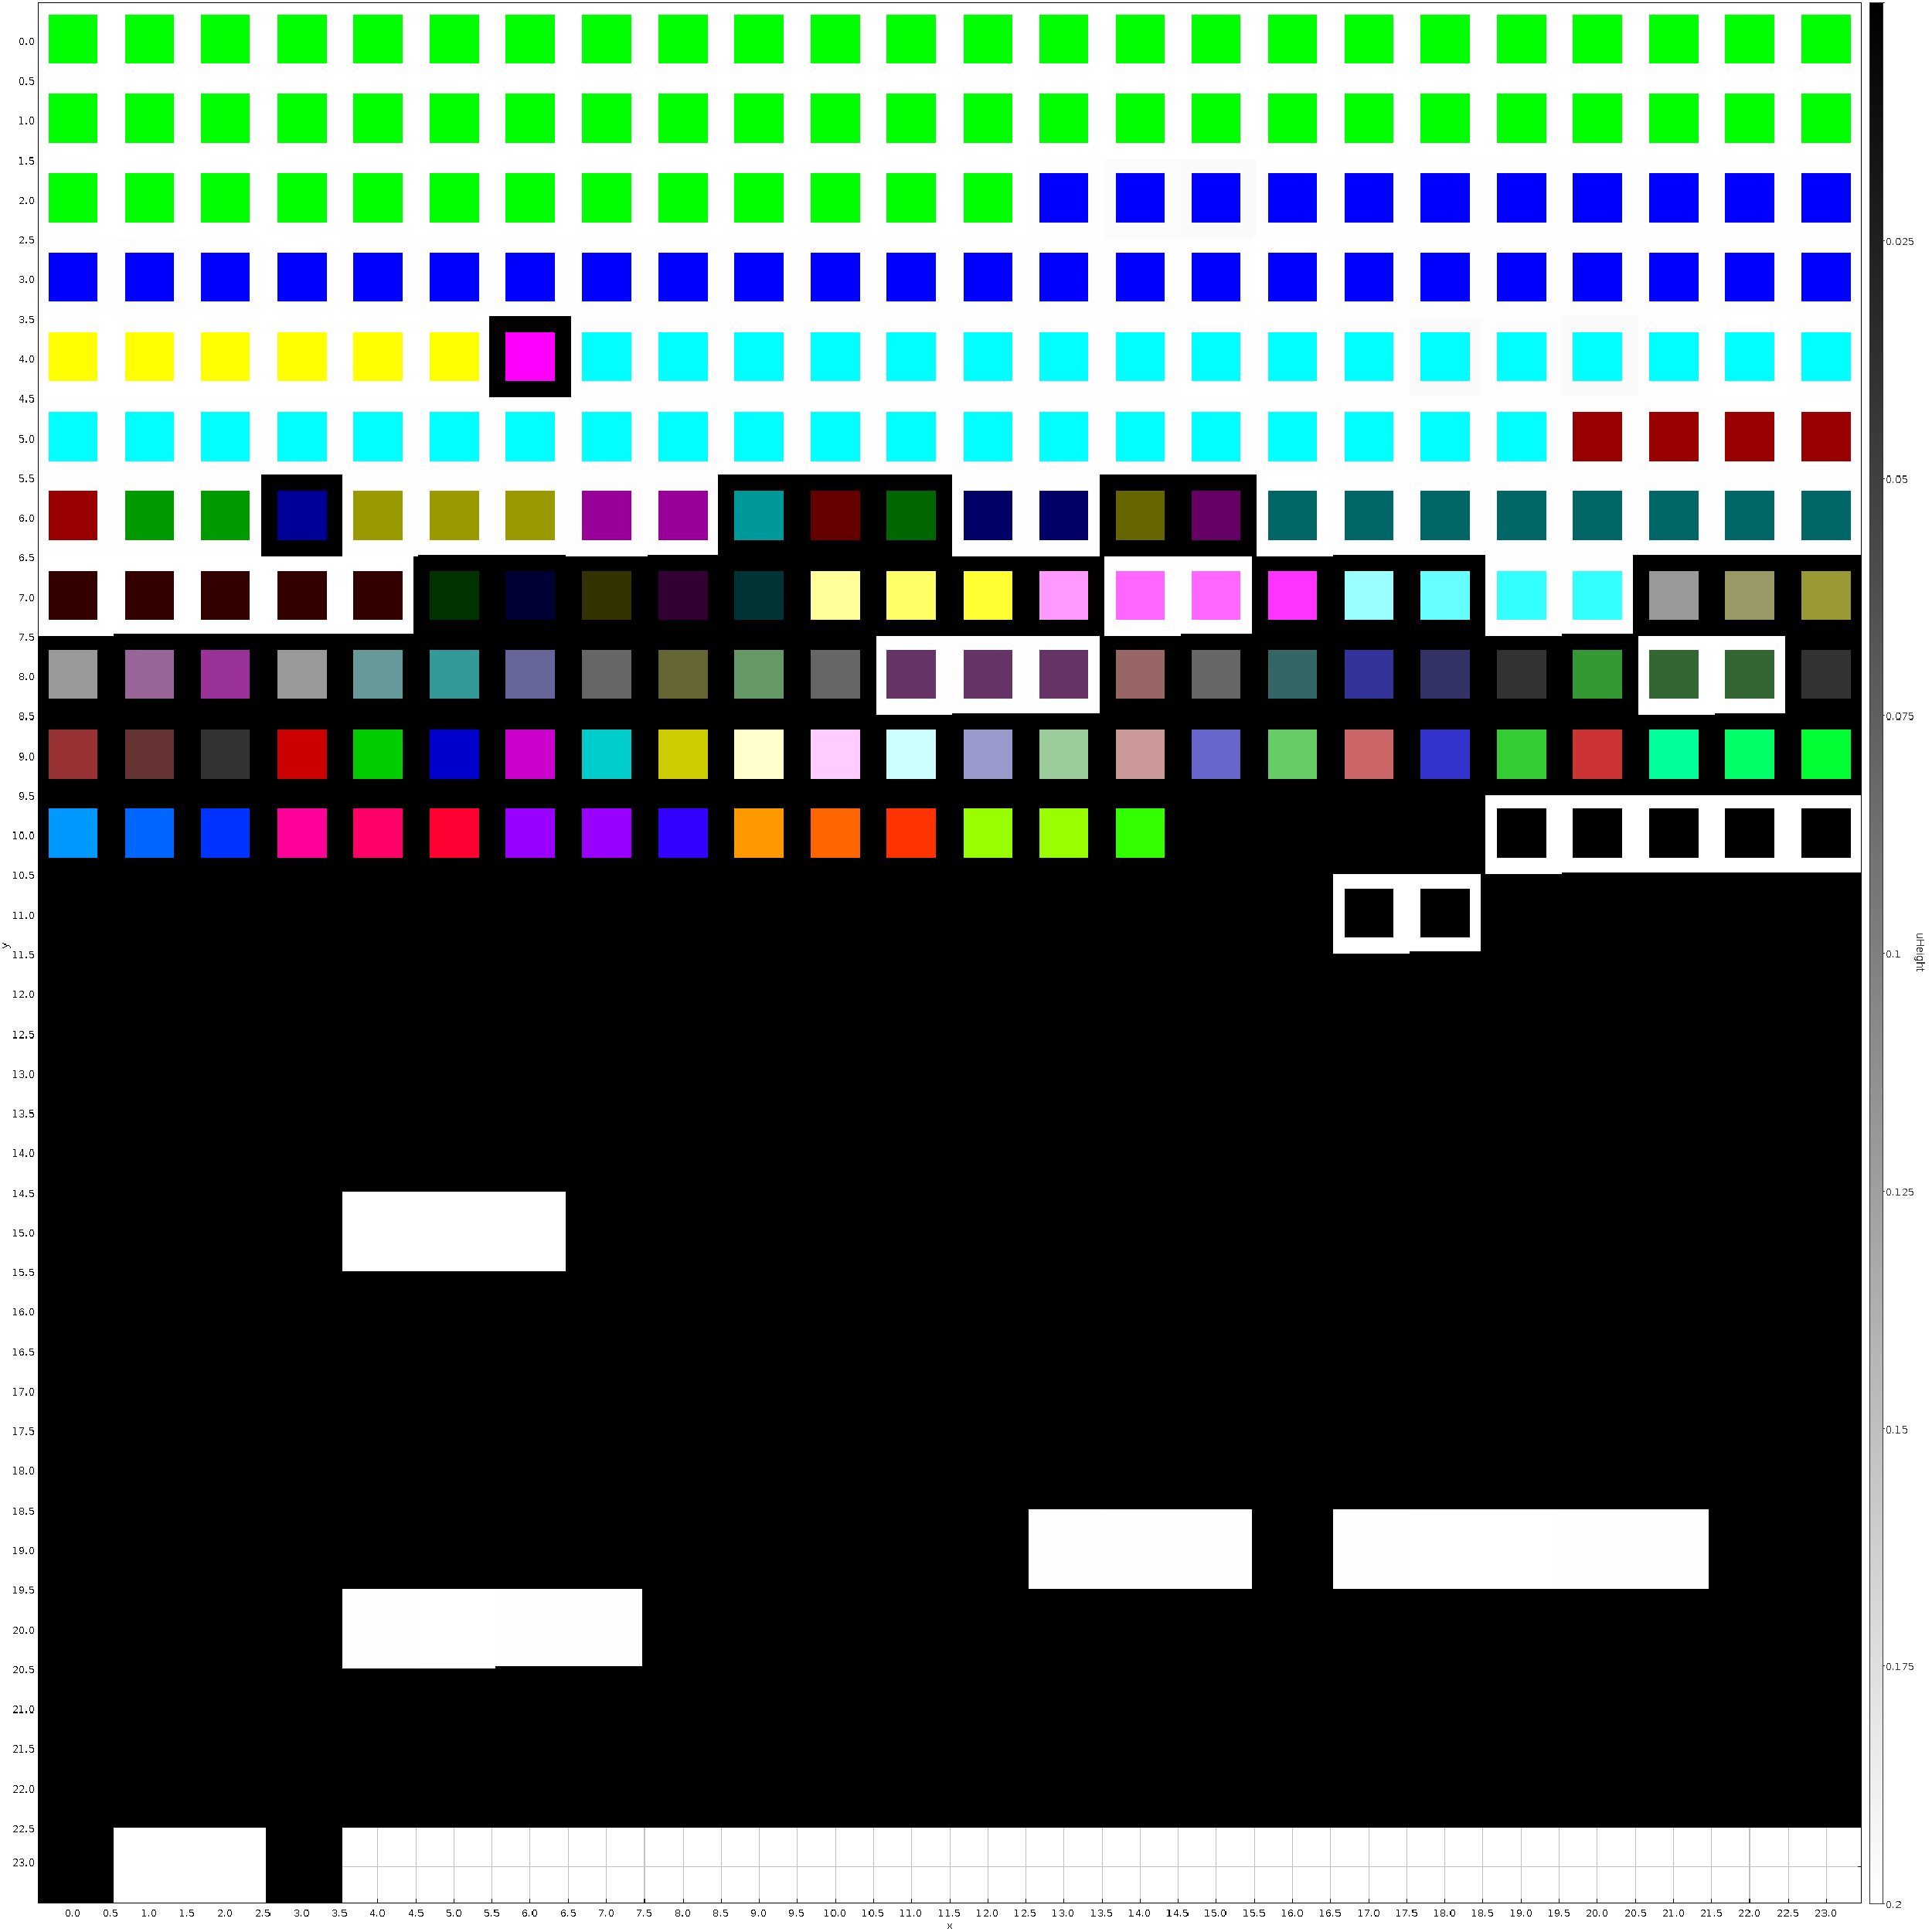
\includegraphics[width=0.31\textwidth]{matri6-01.png}
    \caption{All of the images correspond to U-matrices of the ended experiments mentioned above in order (Train2, Train3, Train6)}
    \label{img:matrixended}
\end{figure}
 There is work to be done for this cases, understand what is going on and interpret correctly the results, but last we got some.
\subsection{CSOM}
%one image
Well, as I mentioned before I did some tests using the ESOM method but since I wasn't getting any results I thought of testing this method, as always I strongly recommend to read carefully its manual, \url{http://dame.dsf.unina.it/documents/SOFM_UserManual_DAME-MAN-NA-0014-Rel1.1.pdf} and fully understand what is going on behind the curtains. In the meanwhile, this is my own explanation. This method uses FITS files, does not support data cubes, specifically uses a neighbourhood function in order to preserve the topological properties of the input space, it is a type of artificial network and is mainly unsupervised learning  and produces a low dimensional discretized representation of the input space of the training samples. I in this case you can choose the number of clusters/neurons in the first layer (neural network), the diameter, number of layers (in the neural network), learning rate and variance  on each layer. Here you have more input parameters to control.
\subsubsection{Expected Results}
Well in this case, since only FITS images are allowed, what we expect to find are areas identifying the different objects in the interstellar medium.

The important results in this case, are got in the \emph{Run} and \emph{Test} steps, in the \emph{Train} step only the network configuration is outputted. What we are interested on seeing are the plotted clusters.
\subsubsection{Tests}
In this case I did some tests on the CSOM workspace, but none of the, where successful, too many input variables to control and test. So, in this case I will leave this parameters free for you to try. I do believe that this method could be very useful and if you find a way to input the data cube in a different configuration you will get some interesting results, due to the fact that in this method the preservation of the topology is one of the main principles.

\section{Further work}
Well, finally we reached the point where I my time in Canada finished and I this research is still on its first stages. I have so many ideas of how to explore the clustering techniques in the DAME platform, MatLab, Python and everything else that can be tested. 

\subsection{Some interesting ideas}

For now, I would say that your best chance here, is to device an efficient way to input the information contained in a data cube as a list of points with values and reduce its dimensionality by randomly choosing them on every layer. If you are ever stuck, or no new ideas come to your mind, do not hesitate to contact me I might have a new interesting idea you can test.

\subsection{Links you should check out}
Most of them are listed in the useful resources section of The Caltech-JPL Summer School on Big Data Analytics, the web page \url{https://class.coursera.org/bigdataschool-001/wiki/Useful_resources}, you may need to create an account in Coursera and enrol in the course. And the rest of them are located in the References section on my GitHub page, \url{https://github.com/LaurethTeX/Clustering/blob/master/References.md}.
\vfill
\textit{Wish you all the best, Andrea Hidalgo}